\documentclass[12pt]{article}
\setlength{\oddsidemargin}{0in}
\setlength{\evensidemargin}{0in}
\setlength{\textwidth}{6.5in}
\setlength{\parindent}{0in}
\setlength{\parskip}{\baselineskip}

\usepackage{amsmath,amsfonts,amssymb,graphicx}

\title{Your Project Title}

\begin{document}

IBEHS 4A03 \hfill Assignment \#1\\
Baoze Lin, Hady Ibrahim

\hrulefill

% Custom numbering for subparts (e.g., 2.1, 2.2)
\renewcommand{\theenumii}{\arabic{enumi}.\arabic{enumii}}

\begin{enumerate}
\item Question 1
  \begin{enumerate}
  % ANSWER TO 1.1
  \item yapyapyap

  \end{enumerate}
\newpage

\item Question 2
  \begin{enumerate}
  % ANSWER TO 2.1
  \item 

  The ordinary differential equation (ODE) governing the temperature \( T(t) \) is:

  \[
  \frac{dT(t)}{dt} = \frac{Q_f(t) - UA(T(t) - T_a)}{\rho V c_p}
  \]

  For this problem, the furnace is off, so \( Q_f(t) = 0 \). Substituting this into the equation:

  \[
  \frac{dT(t)}{dt} = \frac{-UA(T(t) - T_a)}{\rho V c_p}
  \]

  At steady state, the temperature \( T(t) \) no longer changes with time, so:

  \[
  \frac{dT(t)}{dt} = 0
  \]

  Substitute this condition into the ODE:

  \[
  0 = \frac{-UA(T(t) - T_a)}{\rho V c_p}
  \]

  Solve:

  \[
  T(t) - T_a = 0
  \]

  Thus:

  \[
  T(t) = T_a
  \]

  % ANSWER TO 2.2
  \item 
    Using the dervied equation for \( T(t) \), the behaviour of the furnace as defined below, and the given definition of one step of the univariate Euler's method, we can plot Figure 1.

  \[
  Q_f(t) =
  \begin{cases} 
  0 & \text{When } T(t) > 23^\circ \text{C}, \\
  1.5 \times 10^6 & \text{When } T(t) < 17^\circ \text{C}, \\
  \text{unchanged} & \text{For all } 17 \leq T(t) \leq 23^\circ \text{C}.
  \end{cases}
  \]

  \begin{figure}[h!]
    \centering
    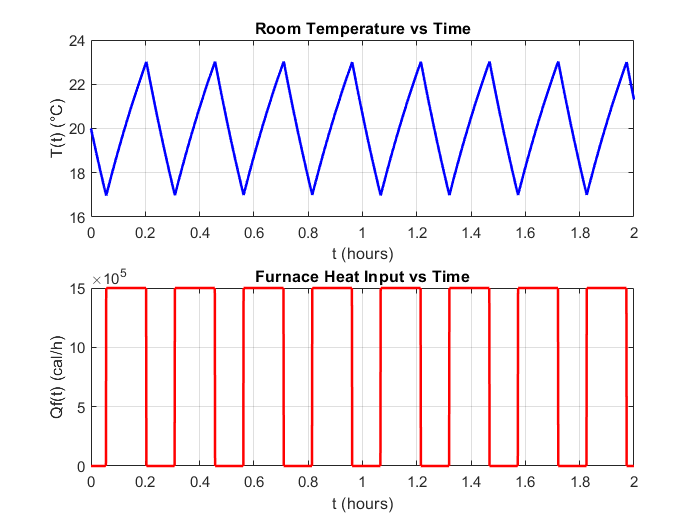
\includegraphics[width=0.8\textwidth]{Figures/figure21.png}
    \caption{Temperature and Furnace Input Over Time}
    \label{fig:figure21} 
  \end{figure}

  \end{enumerate}
\newpage

\item Question 3
  \begin{enumerate}
  \item Part A  % This will appear as "3.1"

  SOLUTION

  \item Part B  % This will appear as "3.2"

  SOLUTION
  \end{enumerate}
\newpage

\item Question 4
  \begin{enumerate}
  \item Part A  % This will appear as "4.1"

  SOLUTION

  \item Part B  % This will appear as "4.2"

  SOLUTION
  \end{enumerate}
\newpage

\item Question 5
  \begin{enumerate}
  \item Part A  % This will appear as "5.1"

  SOLUTION

  \item Part B  % This will appear as "5.2"

  SOLUTION
  \end{enumerate}
\newpage

\end{enumerate}
\end{document}
